\chapter{Appendix \label{Chapter-Appendix}}

\section{Predicted sleep stages \label{Apx-Pred-Hypnogram}}

To obtain sleep stage predictions for our model, we used a pre-trained cardiorespiratory sleep staging model, as described by Bakker et al. \cite{bakker2021estimating}. The model was designed to use any arbitrary combination of input signals to predict the 4-class hypnogram (Wake, combined N1/N2, N3, and REM). We opted to use only the PPG signal to fit our goal. When evaluating against Somnolyzer scorings of the MESA dataset, we achieved a Cohen's Kappa of 0.57, showing moderate agreement. Table \ref{tab:predicted-hypnogram-results} shows additional metrics and classification tasks, like a binary wake versus sleep task.

The performance is lower than reported in the original paper, which is due to the fact that they used additional input signals.Combining cardiac information with airflow, their algorithm reached a Kappa of 0.643 in 4-class classification and 0.680 when also incorporating respiratory effort.

\renewcommand{\arraystretch}{1.5}
\begin{table}[h!]
    \centering
    \begin{tabular}{ p{2.5cm} p{2cm} p{2.3cm} p{2.3cm} p{1.5cm} p{2.3cm} }
        Task & Kappa & Acc. & Se. & Sp. & PPV \\
        \hline
        4-cl. \newline (Wake/N1-\newline N2/N3/REM) & 0.566 \newline [0.436, 0.677] & 73.2\%\newline [64.8\%, 80.0\%] & - & - & - \\
        3-cl. \newline (Wake/NREM\newline/REM) & 0.628 \newline [0.473, 0.740] & 79.4\%\newline [70.8\%, 85.6\%] & - & - & - \\
        2-cl. \newline (Wake/Sleep) & 0.653 \newline [0.475, 0.778] & 84.6\% \newline [76.2\%, 90.3\%] & 73.1\% \newline [56.9\%, 84.9\%] & 91.8\% \newline (8.37\%) & 89.6\% \newline [79.0\%, 95.2\%] \\
    \end{tabular}
    \caption{PPG-based sleep stage prediction performances against Somnolyzer scorings on different tasks. Values are presented as median and 25th and 75th percentiles, median [Q1, Q2], or (in case of normally distributed data) as mean and standard deviation, mean (sd). \label{tab:predicted-hypnogram-results}}
\end{table}

Figure \ref{fig:tst-plot} shows the true TSTs from Somnolyzer plotted against the predicted TSTs and the Bland-Altman-Plot. The sleep stage predictor achieved a RMSE of 1.1 (hours) and a Spearman rank correlation of 0.712.

\begin{figure}
    \centering
    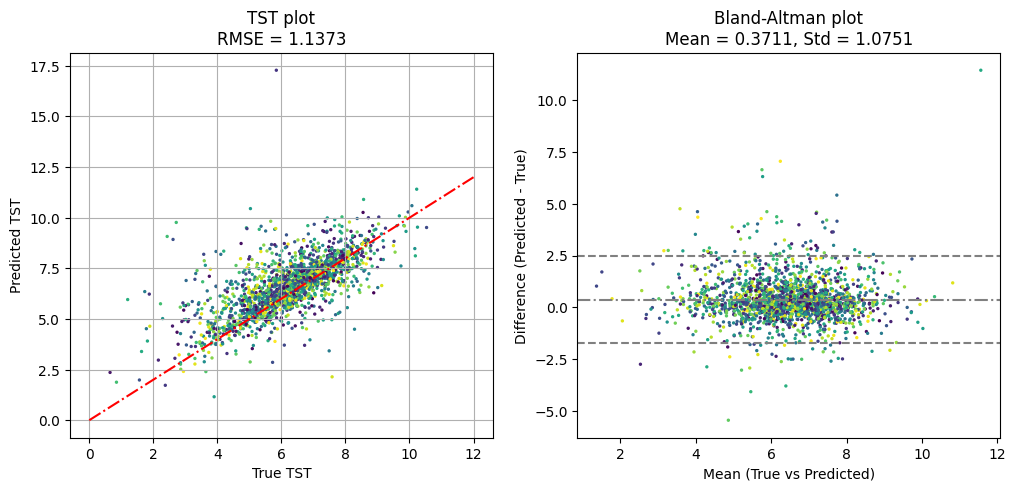
\includegraphics[width=\textwidth]{images/TstPlot}
    \caption{Predicted TST plotted against the true TST from Somnolyzer (left) and the Bland-Altman-Plot (right). The red line is the identity line. The upper and lower gray lines show the levels of agreement.}
    \label{fig:tst-plot}
\end{figure}

\section{Lowpass denoising of the PPG signal \label{Apx-Denoise}}

\begin{figure}[h!]
    \centering
    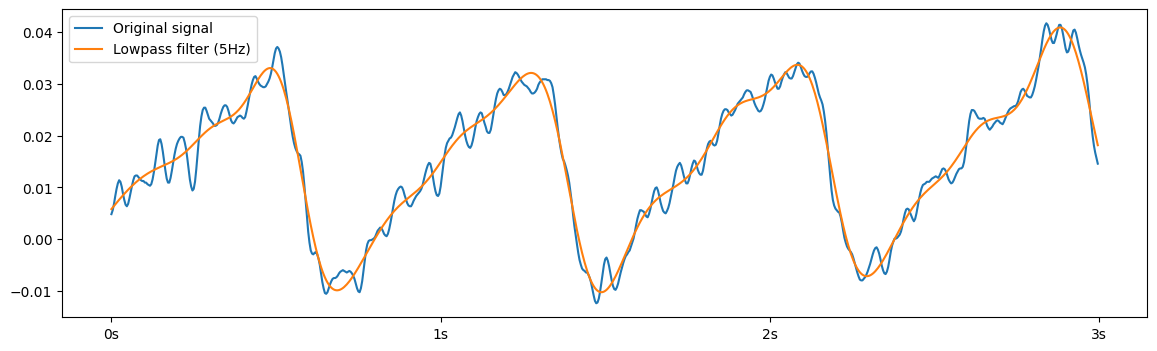
\includegraphics[width=\textwidth]{images/Lowpass}
    \caption{Comparison of the original signal (blue) and the denoised signal (orange) for a random 3-second PPG window from our dataset. We used a lowpass filter with a cutoff frequency of 5Hz.}
    \label{fig:lowpass-example}
\end{figure}

\section{Near-boundary double-labeling \label{Apx-NBL}}

In NBL, single AHIs can get assigned to a second severity class, if they are near the boundaries. The specific values are as follows:

\renewcommand{\arraystretch}{1.5}
\begin{table}[h!]
    \centering
    \begin{tabular}{ l c c }
        Severity class & Hard boundaries & NBL boundaries \\
        \hline
        Normal   & $ AHI < 5 $         & $ AHI < 7 $             \\
        Mild     & $ 5 \le AHI < 15 $  & $ 2.4 \le AHI < 17.4 $  \\
        Moderate & $ 15 \le AHI < 30 $ & $ 12.4 \le AHI < 35.2 $ \\
        Severe   & $ 30 \le AHI $      & $ 26.6 \le AHI $        \\
    \end{tabular}
\end{table}

\section{Severity-class-level metrics \label{Apx-Severity-Metrics}}

\renewcommand{\arraystretch}{1.5}
\begin{table}[h!]
    \centering
    \begin{tabular}{p{3cm} p{3cm} p{4cm}}
        Metric & Calculation & Meaning \\
        \hline
        Accurracy \newline (Acc) & $\frac{TP+TN}{TP+FP+FN+TN}$ & What \% got \newline correctly classified? \\
        Sensitivity \newline (Se, alt. Recall) & $\frac{TP}{TP+FN}$ & What \% of positives \newline got correctly \newline classified? \\
        Specificity \newline (Sp) & $\frac{TN}{TN+FP}$ & What \% of negatives \newline got correctly \newline classified? \\
        Positive Predicted \newline Value (PPV) & $\frac{TP}{TP+FP}$ & What \% of predicted \newline positives where \newline really positive? \\
        Negative Predicted \newline Value (NPV) & $\frac{TN}{TN+FN}$ & What \% of predicted \newline negatives where \newline really negative? \\
    \end{tabular}
\end{table}

\section{Example model output \label{Apx-Output}}

\todo{FIGURE, Top and bottom rows show the true labels (event or not); second row show the predicted probabilities of the models sigmoid layer; third row shows an applied example threshold of ???; fourth row shows the thresholded predictions after the correction step. One can see, that ....}